\section{\texorpdfstring{Backgrounds for $\tauTau$}{Backgrounds for tauTau}}
\label{sect:bkg}
\subsection{QCD multi-jet background estimation in tauTau channel}
%In this section, data driven methods are applied to estimate the contribution of
% the main backgrounds in the signal region.
In QCD multi-jet events all tau candidates are misidentified as jets. Due to the large cross
section and
the poor MC modelling of the tau misidentification rate from jets, the QCD multi-jet contribution in the signal region 
is estimated from data using the ABCD method.
This method relies on different distributions of QCD
in the four exclusive regions labelled as A, B, C (the control regions) and D (the signal region) which are defined in a two-dimensional plane as a function of uncorrelated discriminating variables.
Then the number of QCD events in signal region D can be calculated from the number of QCD events in the control region A multiplied by a transfer factor which is defined as the ratio of the number of QCD events in the control region C to the number of QCD events in control region B$(T=C/B)$.\\
The two discriminating variables used to define regions A, B, C and D are the isolation 
variable and a kinematic variable chosen as \mttwo in search \binone or \SumMT in search \bintwo.  
The definitions of the control regions are summarized in Table~\ref{2QCDbg}. \\
The distribution of the transfer factor as a 
function of the search variable is shown in Figure~\ref{fig:1QCDbg}. The correlation 
between the two variables used to define the four exclusive regions is marginal, since the ratio plots can be fit with a straight line using a $pol0$ function. The fit function is also shown in the plots. 
\begin{figure}[htbp]
\centering
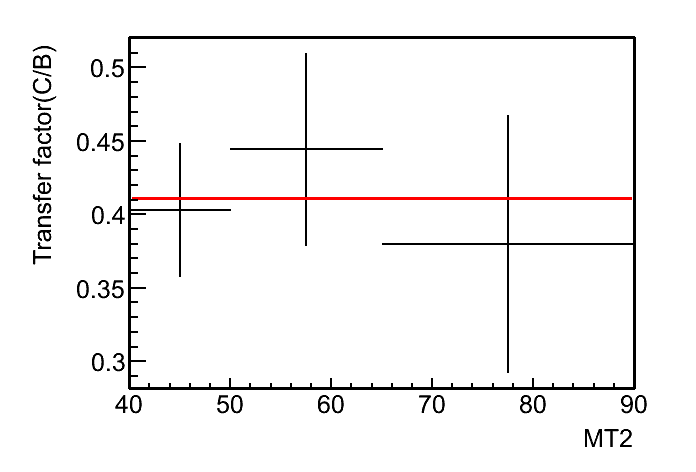
\includegraphics[width=0.49\textwidth]{QCDbginTauTau/Bin1_transferfactor.png}
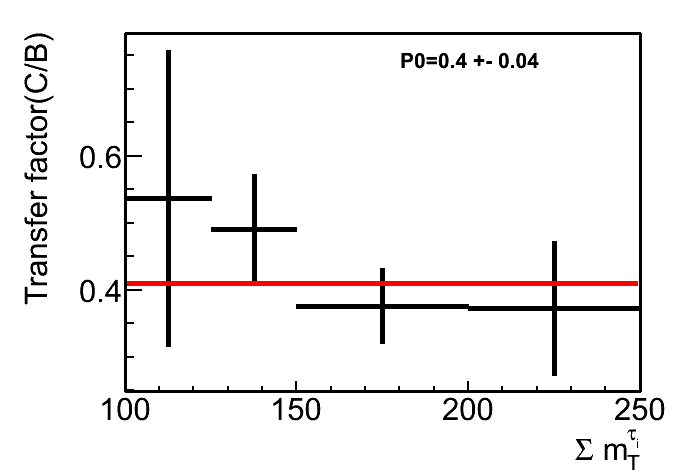
\includegraphics[width=0.49\textwidth]{QCDbginTauTau/Bin2_transferfactor.png} \\
\caption{The distribution of transfer factor as a function of \mttwo (left) and \SumMT (right). A $pol0$ function is used to fit the plots.}
\label{fig:1QCDbg}
\end{figure}
\begin{table}
\begin{center}
\begin{tabular}{|c|c|c|c|}
\hline
Region&A& B & C
\\ \hline\hline
\multirow{5}{*}{search \binone} &$\mttwo >90$ & $\mttwo <90$&$\mttwo <90$ \\
&at least 1 loose taus&at least 1 loose taus& loose tau veto\\
&loose-loose loose-medium &loose-loose loose-medium &medium-medium \\
&loose-tight&loose-tight&medium-tight tight-tight\\
&No cut on charge&No cut on charge& OS\\
\hline
\multirow{5}{*}{search \bintwo}&$\SumMT >250$ &$\SumMT <250$&$\SumMT < 250$\\
&at least 1 loose taus&at least 1 loose taus& loose tau veto\\
&loose-loose loose-medium &loose-loose loose-medium &medium-medium \\
&loose-tight&loose-tight&medium-tight tight-tight\\
&No cut on charge&No cut on charge& OS\\
% &misc.MinMetJetDphiPt40$>$1 is relaxed\\
\hline
\end{tabular}
\caption{The control regions used for ABCD method are defined. The $\mindphifour>1$ cut is removed to incraese the statistics.}
\label{2QCDbg}
\end{center}
\end{table}
\\The number of QCD multi-jet events in the control regions is estimated from data after subtraction 
of other SM contributions estimated from MC simulation.
In order to increase the contributions from QCD events, the cut on the $\mindphifour>1$ is removed.
But instead a cut efficiency should be taken into account to evaluate the final estimations. The 
fraction of QCD events with all selection cuts with respect to the QCD events with all selection 
cuts but the $\mindphifour>1$ are shown in Figure~\ref{fig:3QCDbg}.
\begin{figure}[htbp]
\centering
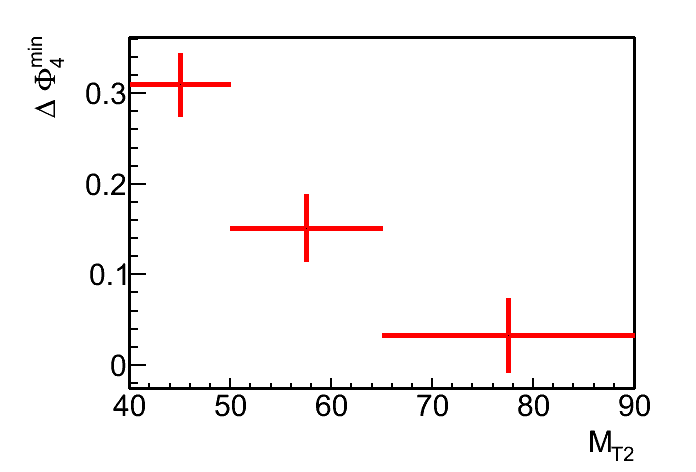
\includegraphics[width=0.49\textwidth]{QCDbginTauTau/Bin1_miscefficiency.png}
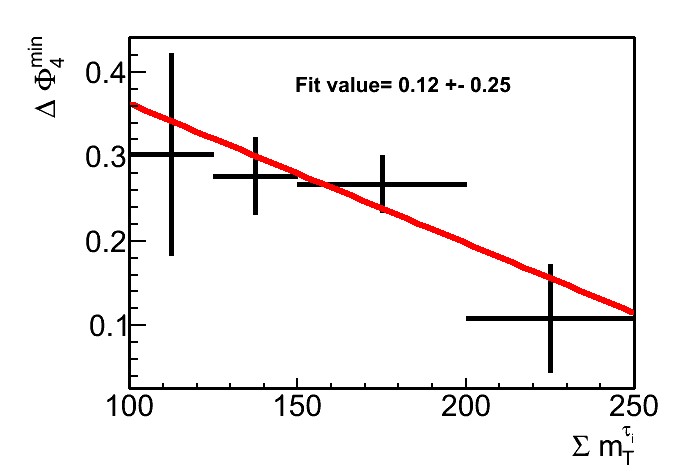
\includegraphics[width=0.49\textwidth]{QCDbginTauTau/Bin2_miscefficiency.png} \\
\caption{ The fraction of QCD events with all selection cuts with respect to the QCD events with all selection 
cuts but the $\mindphifour>1$ as a function of \mttwo (left) and \SumMT (right).}
\label{fig:3QCDbg}
\end{figure}
\\The results of the ABCD method are summarized in table \ref{4QCDbg} and the distributions of the kinematic variables for data, SM backgrounds and SUSY are shown in the Figure~\ref{fig:5QCDbg}. The SM background distributions
are taken from MC simulation, except for the QCD-multi-jet contribution, which is estimated
using the ABCD method.
\begin{table}
\begin{center}
\begin{tabular}{|l|c|c|c|c|c|c|c|}
\hline
& Sample & RegionA & RegionB & RegionC & T=C/B & Estimation \\\hline\hline
\multirow{7}{*}{Bini \mttwo$>$90}& Data&10.00 +- 3.16 & 880.00 +- 29.66& 430.00 +- 20.74& \multirow{7}{*}{0.43+-0.32} & \multirow{7}{*}{0.06 +- 0.08}\\ \cline{2-5}
&Z+jets& 2.27 +- 0.90 &29.27 +- 3.22 & 51.45 +- 4.43 & & \\\cline{2-5}
&W+jets& 2.90 +- 1.43&69.20 +- 8.70 &49.25 +- 7.22 & & \\\cline{2-5}
&WW+jets&0.12 +- 0.07 &0.76 +- 0.17 &1.60 +- 0.25 & & \\\cline{2-5}
&Top& 0.49 +- 0.47&21.78 +- 3.13 & 14.51 +- 2.63& & \\\cline{2-5}
&QCD& 4.23 +- 3.62 & 758.99+-31.24& 313.19+-22.55& & \\\cline{2-5}
&Susy& 1.46 +- 0.17& 3.96 +- 0.28& 9.01 +- 0.41& & \\\cline{2-5}
\hline\hline
\multirow{7}{*}{Binii $\SumMT>250$}&Data &25.00 +- 5.00 &723.00 +- 26.89 &348.00 +- 18.65 & \multirow{7}{*}{ 0.41 +- 0.03} & \multirow{7}{*}{0.61 +- 1.55} & \\\cline{2-5}
&Z+jets& 2.22 +- 1.07 & 21.78 +- 2.72 & 39.57 +- 3.94& & \\\cline{2-5}
&W+jets& 4.28 +- 1.46&51.84 +- 7.48 & 40.09 +- 6.82& & \\\cline{2-5}
&WW+jets& 0.09 +- 0.05& 0.42 +- 0.13& 0.87 +- 0.19 & & \\\cline{2-5}
&Top&0.42 +- 0.41 &3.07 +- 1.22 & 3.31 +- 1.43& & \\\cline{2-5}
&QCD&18.00 +- 5.33 &645.89+-28.07 & 264.16+-20.30& & \\\cline{2-5}
&Susy& 2.13 +- 0.20&1.18 +- 0.15 & 2.80 +- 0.22& & \\\cline{2-5}
\hline
\end{tabular}
\caption{ The MC predicted backgrounds in the multi-jet control regions, including both the
statistical and systematic uncertainties, and the expected multi-jet contribution,obtained
by subtracting the MC contributions from observed data . Predicted event yields for the
SUSY in the control regions are also shown. The estimated multi-jet contribution
in the SRs is given in the last column.
}
\label{4QCDbg}
\end{center}
\end{table}
\begin{figure}[htbp]
\centering
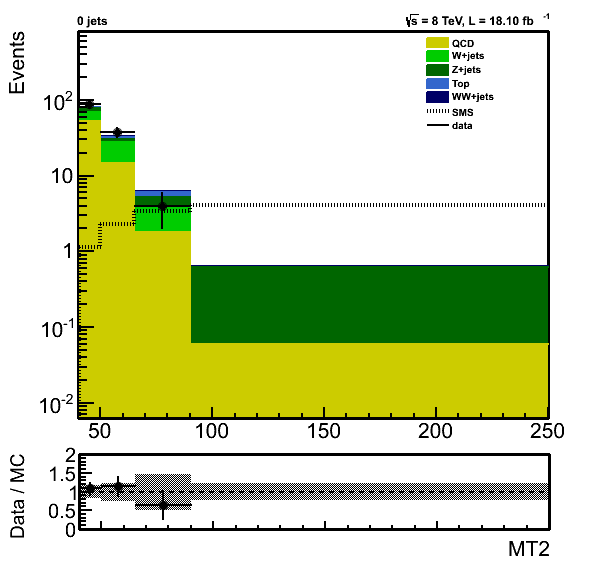
\includegraphics[width=0.49\textwidth]{QCDbginTauTau/Bin1_QCDdatadriven2.png}
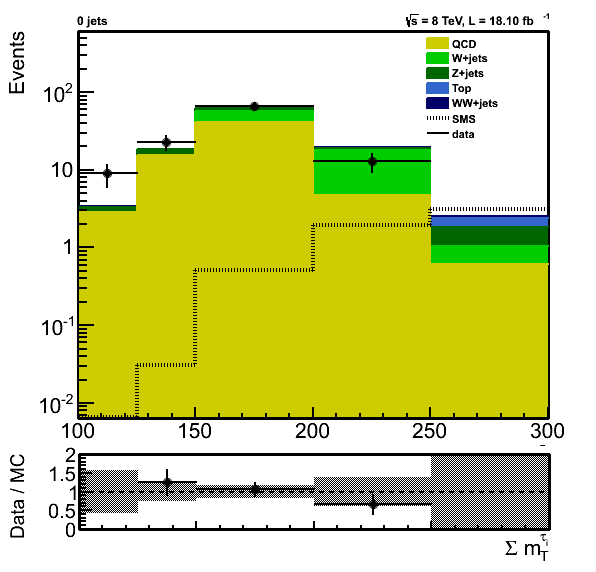
\includegraphics[width=0.49\textwidth]{QCDbginTauTau/Bin2_QCDdatadriven2.png} \\
\caption{Distributions of relevant kinematic variables before the requirement on the given variable
is applied: (a) \mttwo (b) $\SumMT$ . The QCD multi-jet contribution is estimated from data using the ABCD method.}
\label{fig:5QCDbg}
\end{figure}


